% Appendix A

\chapter{Appendix} % Main appendix title

\label{AppendixA} % For referencing this appendix elsewhere, use \ref{AppendixA}
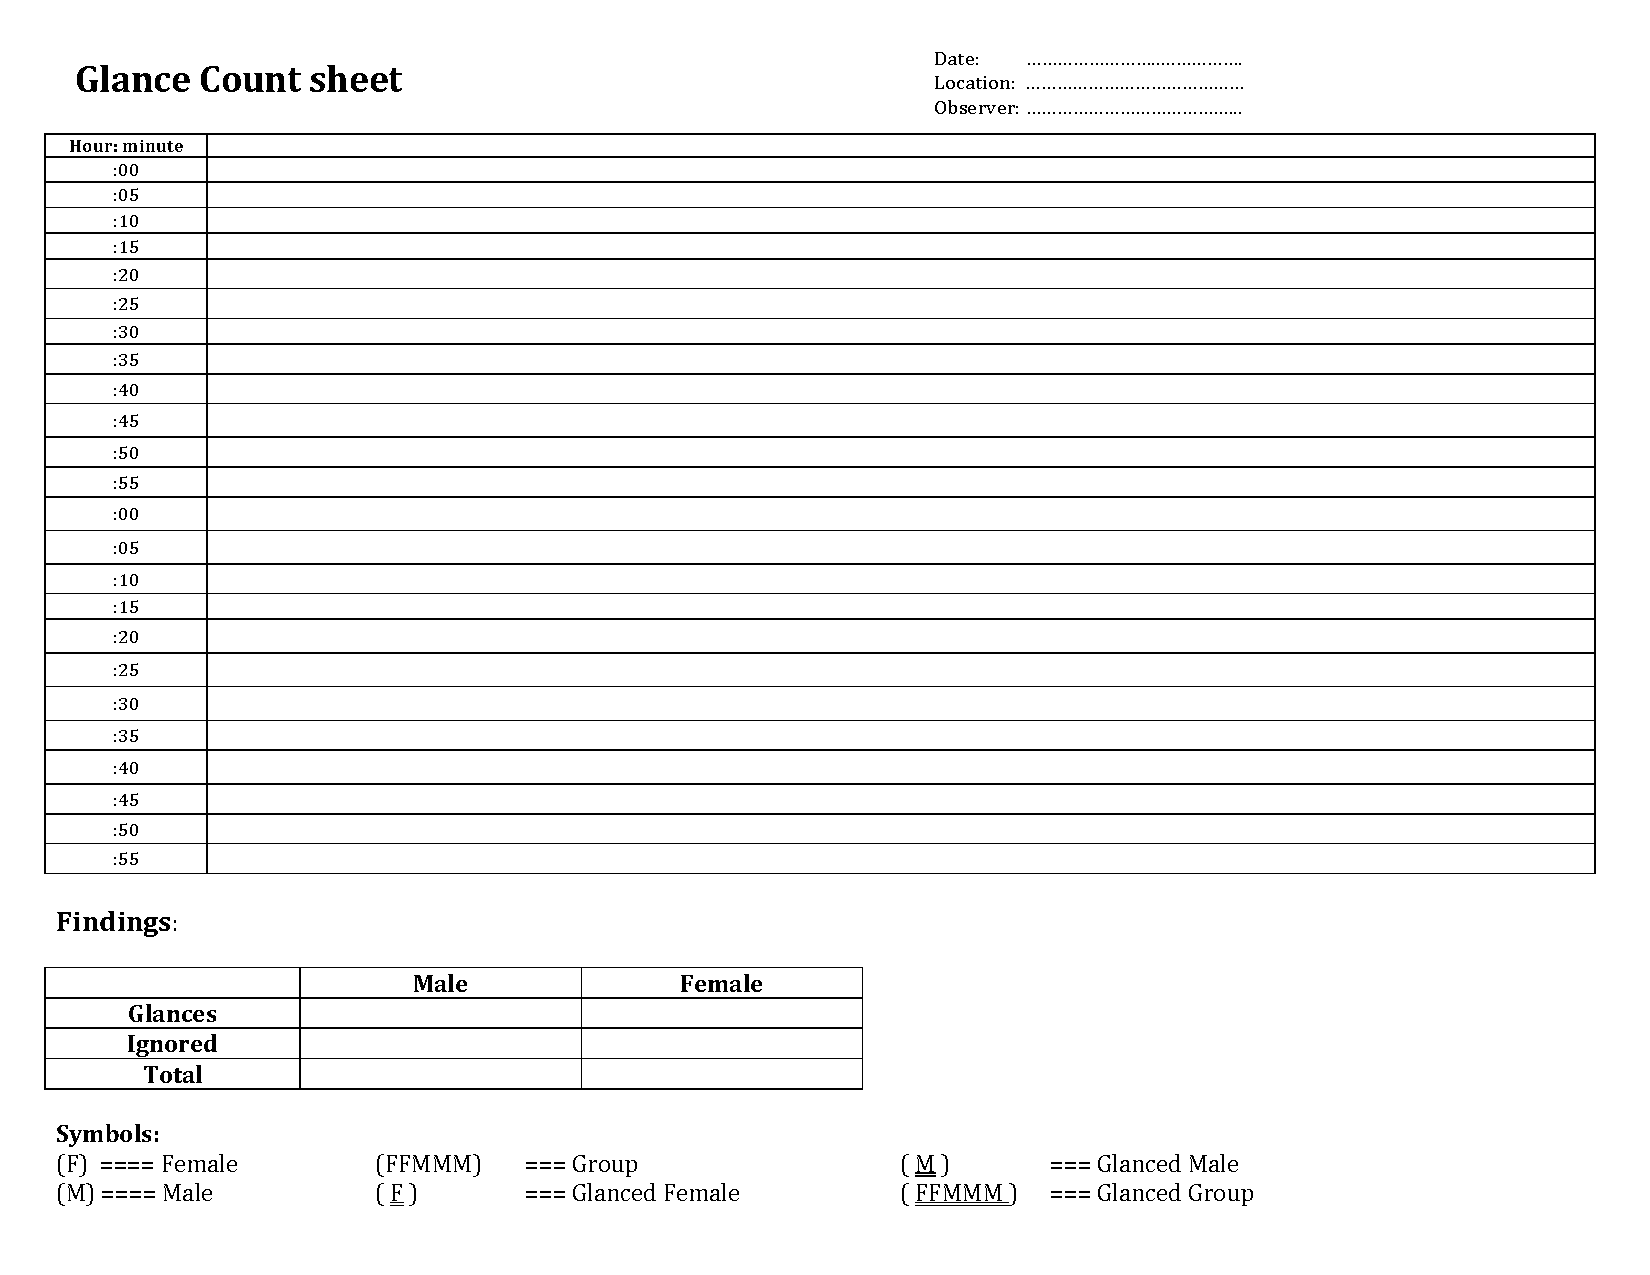
\includepdf[pages=1,width = 15cm, height=20cm,pagecommand=\section{Glance count sheet}]{Appendices/3/Glance_Count_Method.pdf}
\includepdf[pages=1,width = 15cm,pagecommand=\section{Consent Form}]{Appendices/3/Consent_form.pdf}
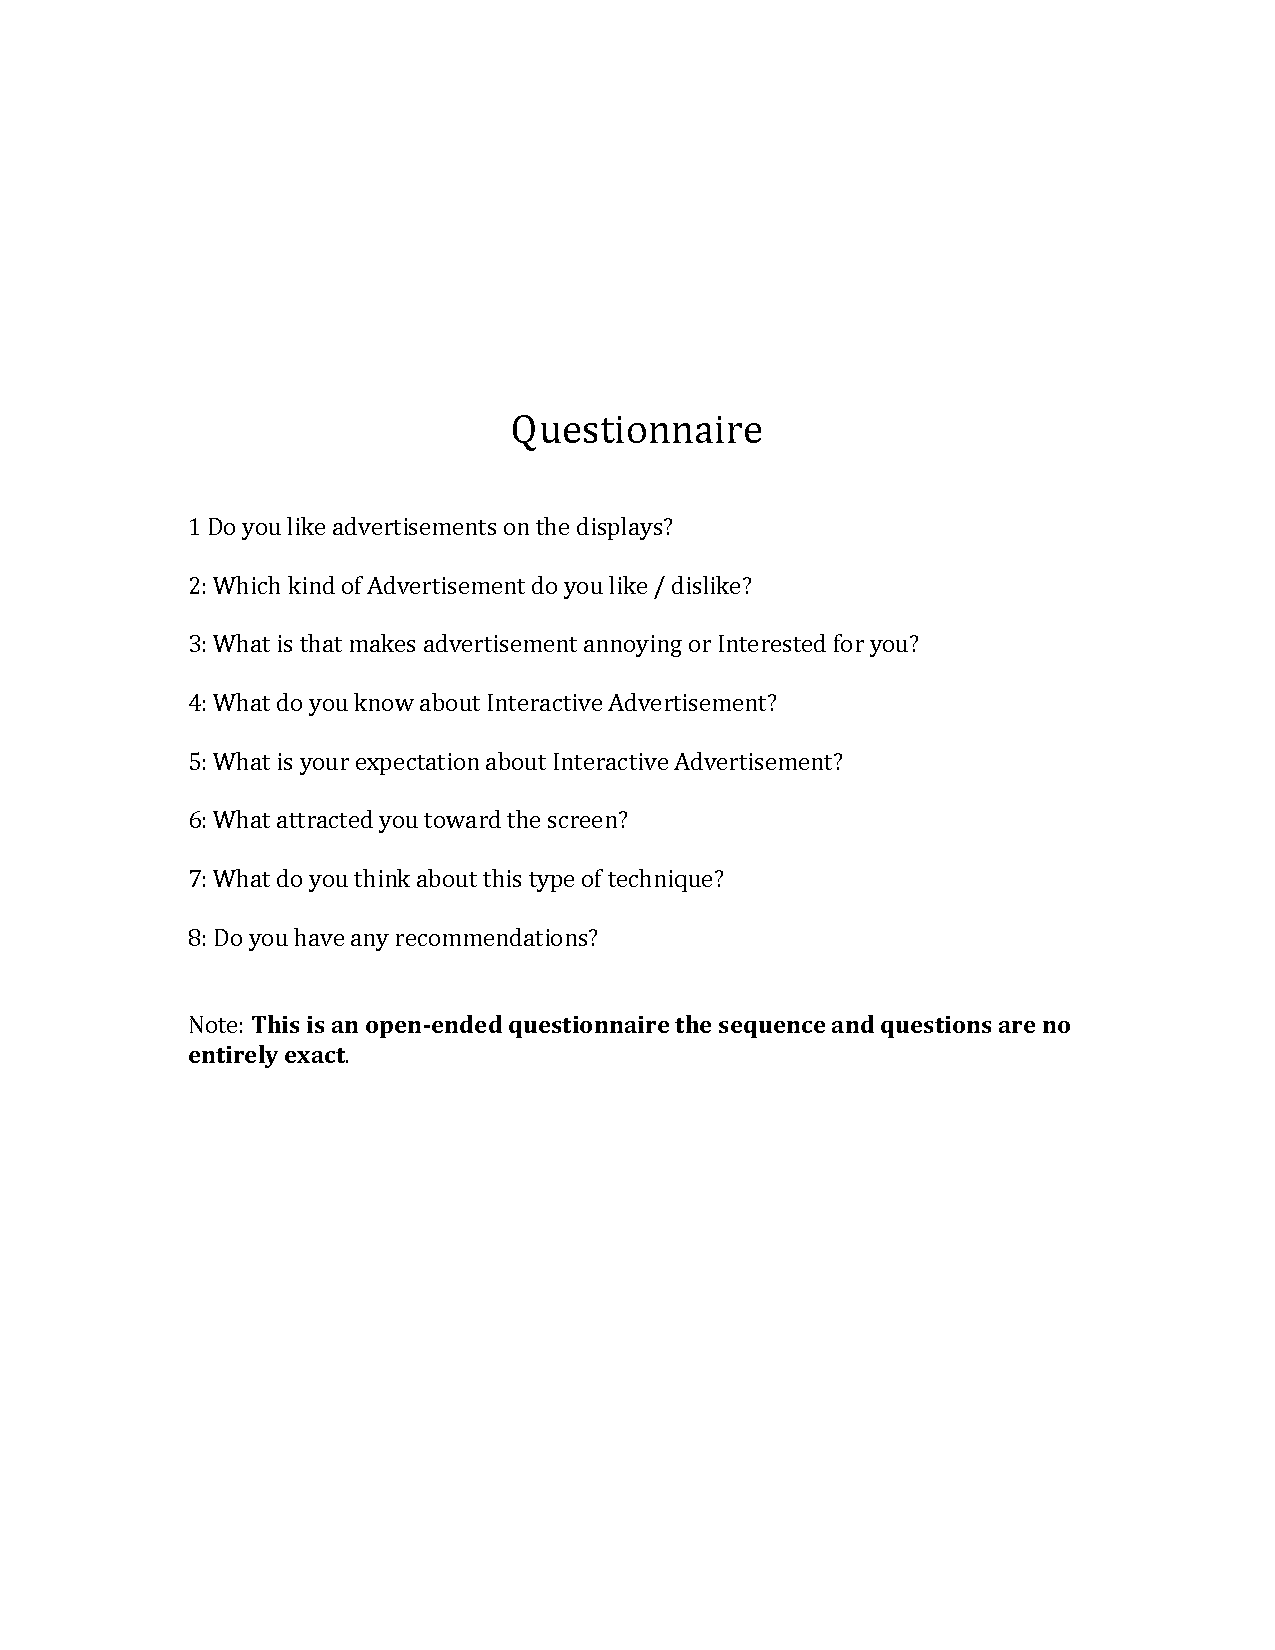
\includepdf[pages=1,width = 15cm, height=20cm,pagecommand=\section{Interview Questionnaire}]{Appendices/3/Questionnaire.pdf}
%\includepdf[scale=0.7,clip,trim=0cm 0cm 0cm 2cm,pages={1},pagecommand={\section{Consent Form}\subsection{part1}}]{Appendices/3/Consent_form.pdf}


\chapter {Focus group skitches}
\label{AppendixB} 
% reset the figure counting
\setcounter{figure}{0}


\begin{figure}[H]
    \centering
    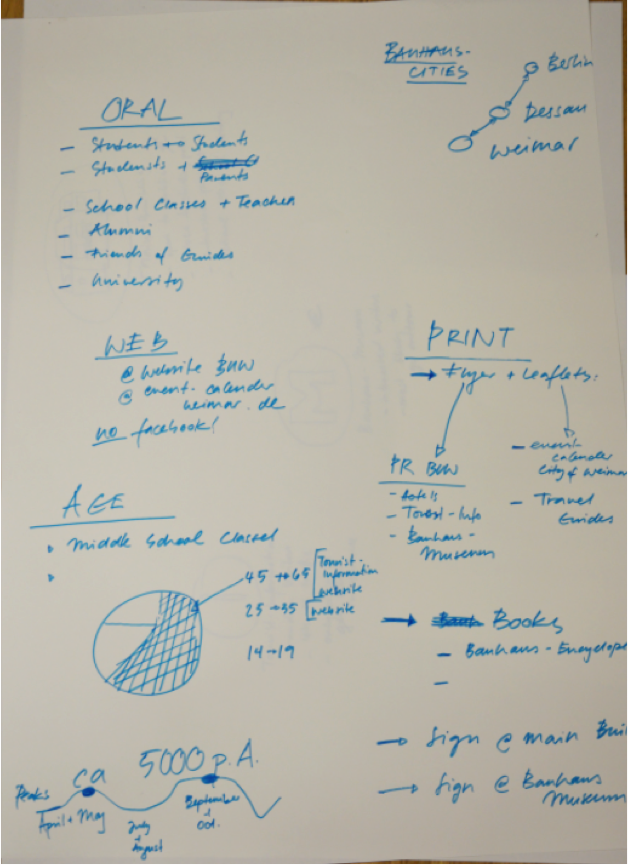
\includegraphics[width=12cm,height=15cm]{Appendices/4/sk1}%
    \caption{First sketch}%
    \label{fig:Sk1}%
\end{figure}


\begin{figure}[H]
    \centering
    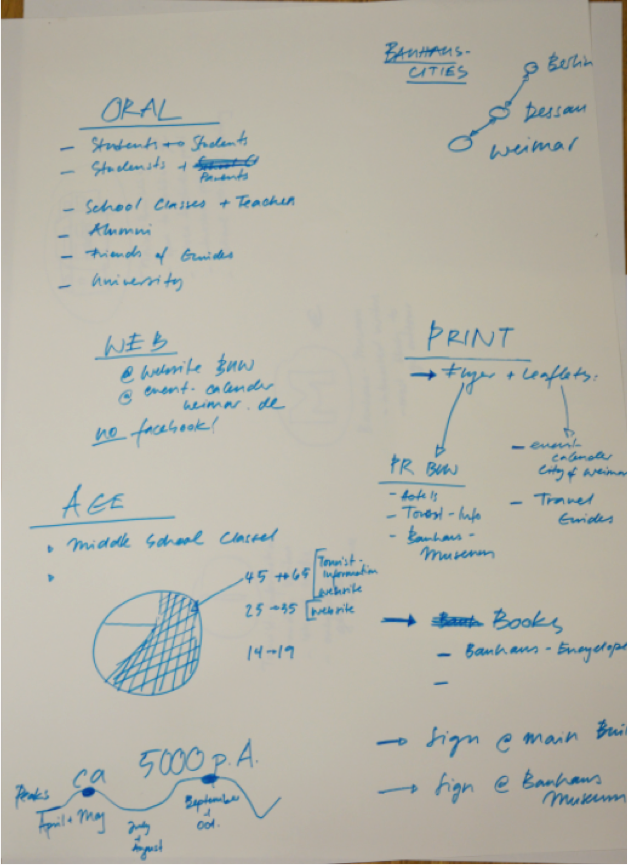
\includegraphics[width=12cm,height=15cm]{Appendices/4/sk2}%
    \caption{Second sketch}%
    \label{fig:Sk2}%
\end{figure}

\begin{figure}[H]
    \centering
    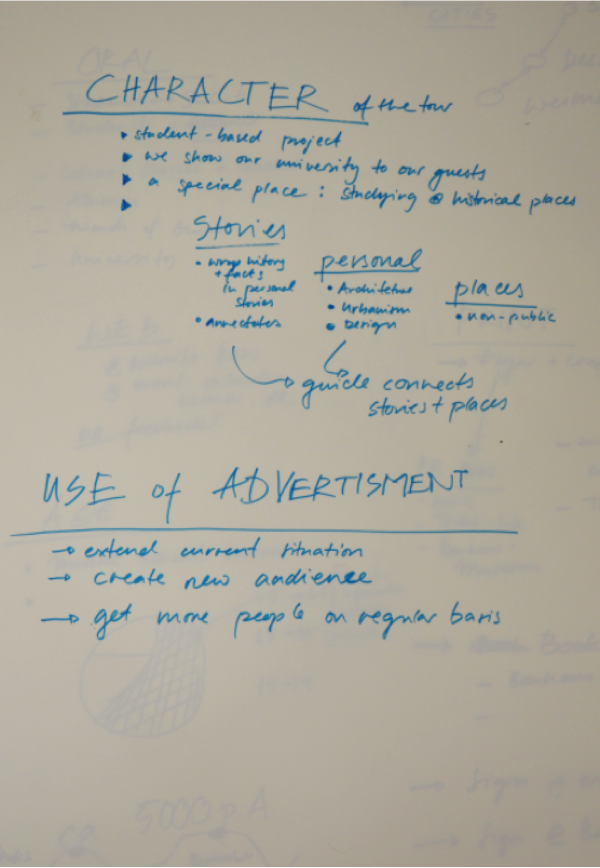
\includegraphics[width=12cm,height=15cm]{Appendices/4/sk3}%
    \caption{Third sketch}%
    \label{fig:Sk3}%
\end{figure}


\chapter {Low fidelity}
\label{AppendixC} 
% reset the figure counting
\setcounter{figure}{0}

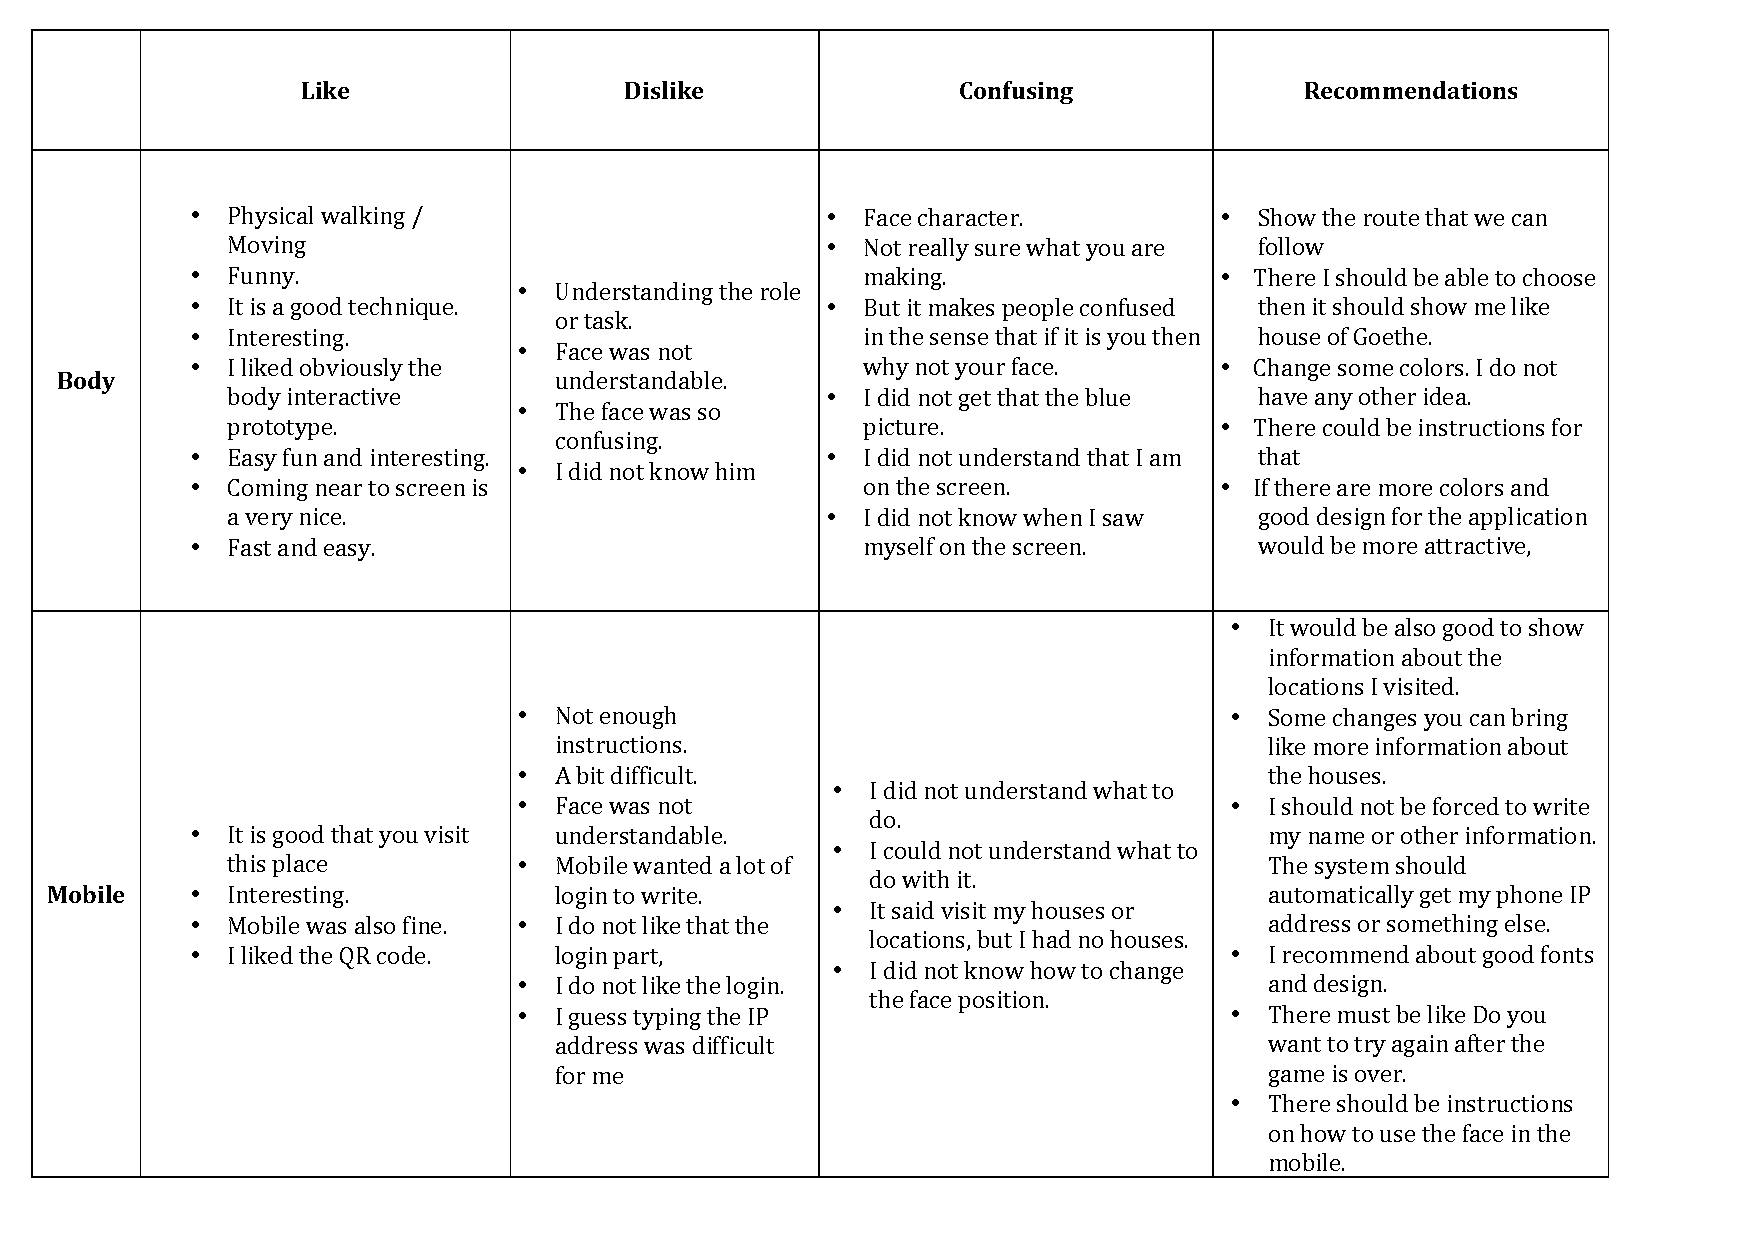
\includepdf[pages=1,width = 20cm, height=15cm,pagecommand=\section{Coded Interviews}]{Appendices/5/Coded_Interview.pdf}


\chapter {Onsite study}
\label{AppendixD} 
\setcounter{figure}{0}
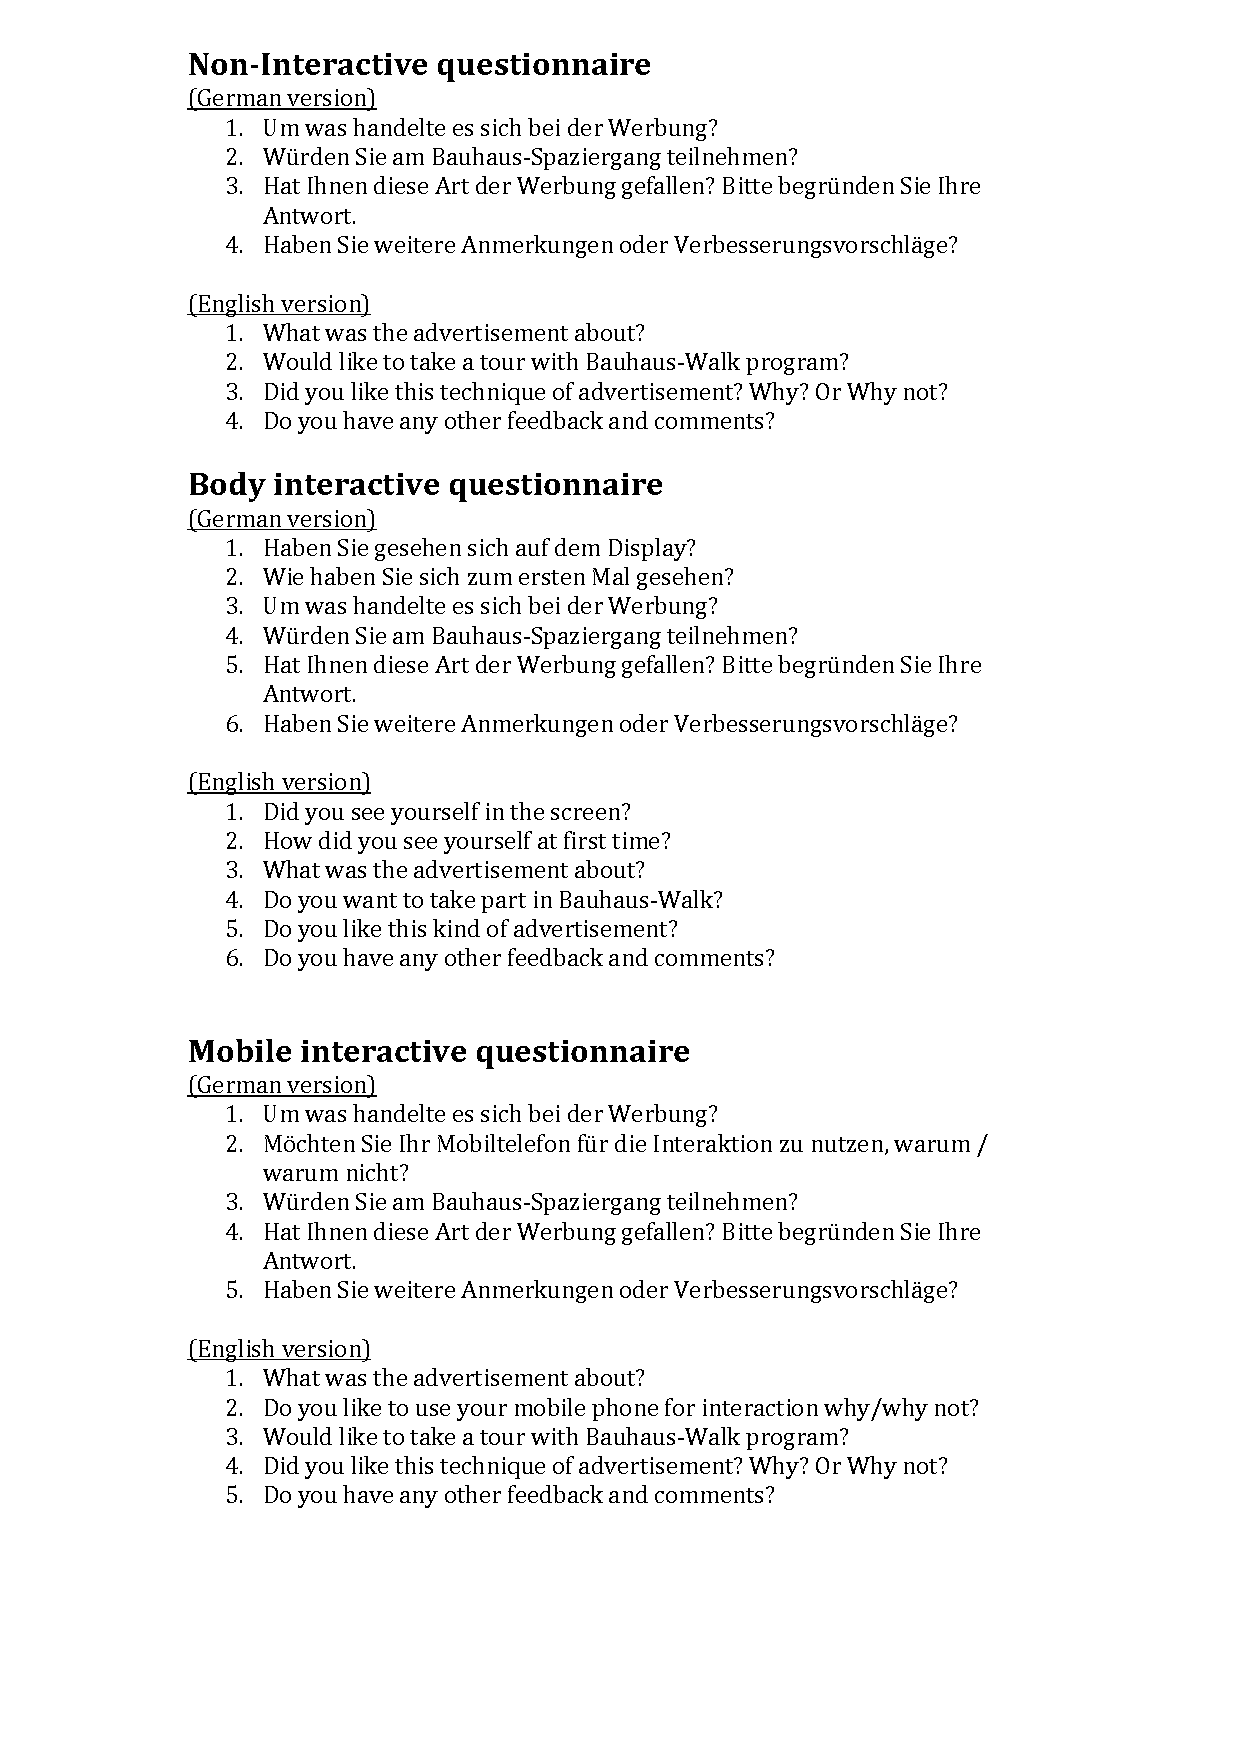
\includepdf[pages=1,width = 20cm, height=22cm,pagecommand=\section{Interview Questionnaire}]{Appendices/8/whole_week_interivew.pdf}



% Glance counts
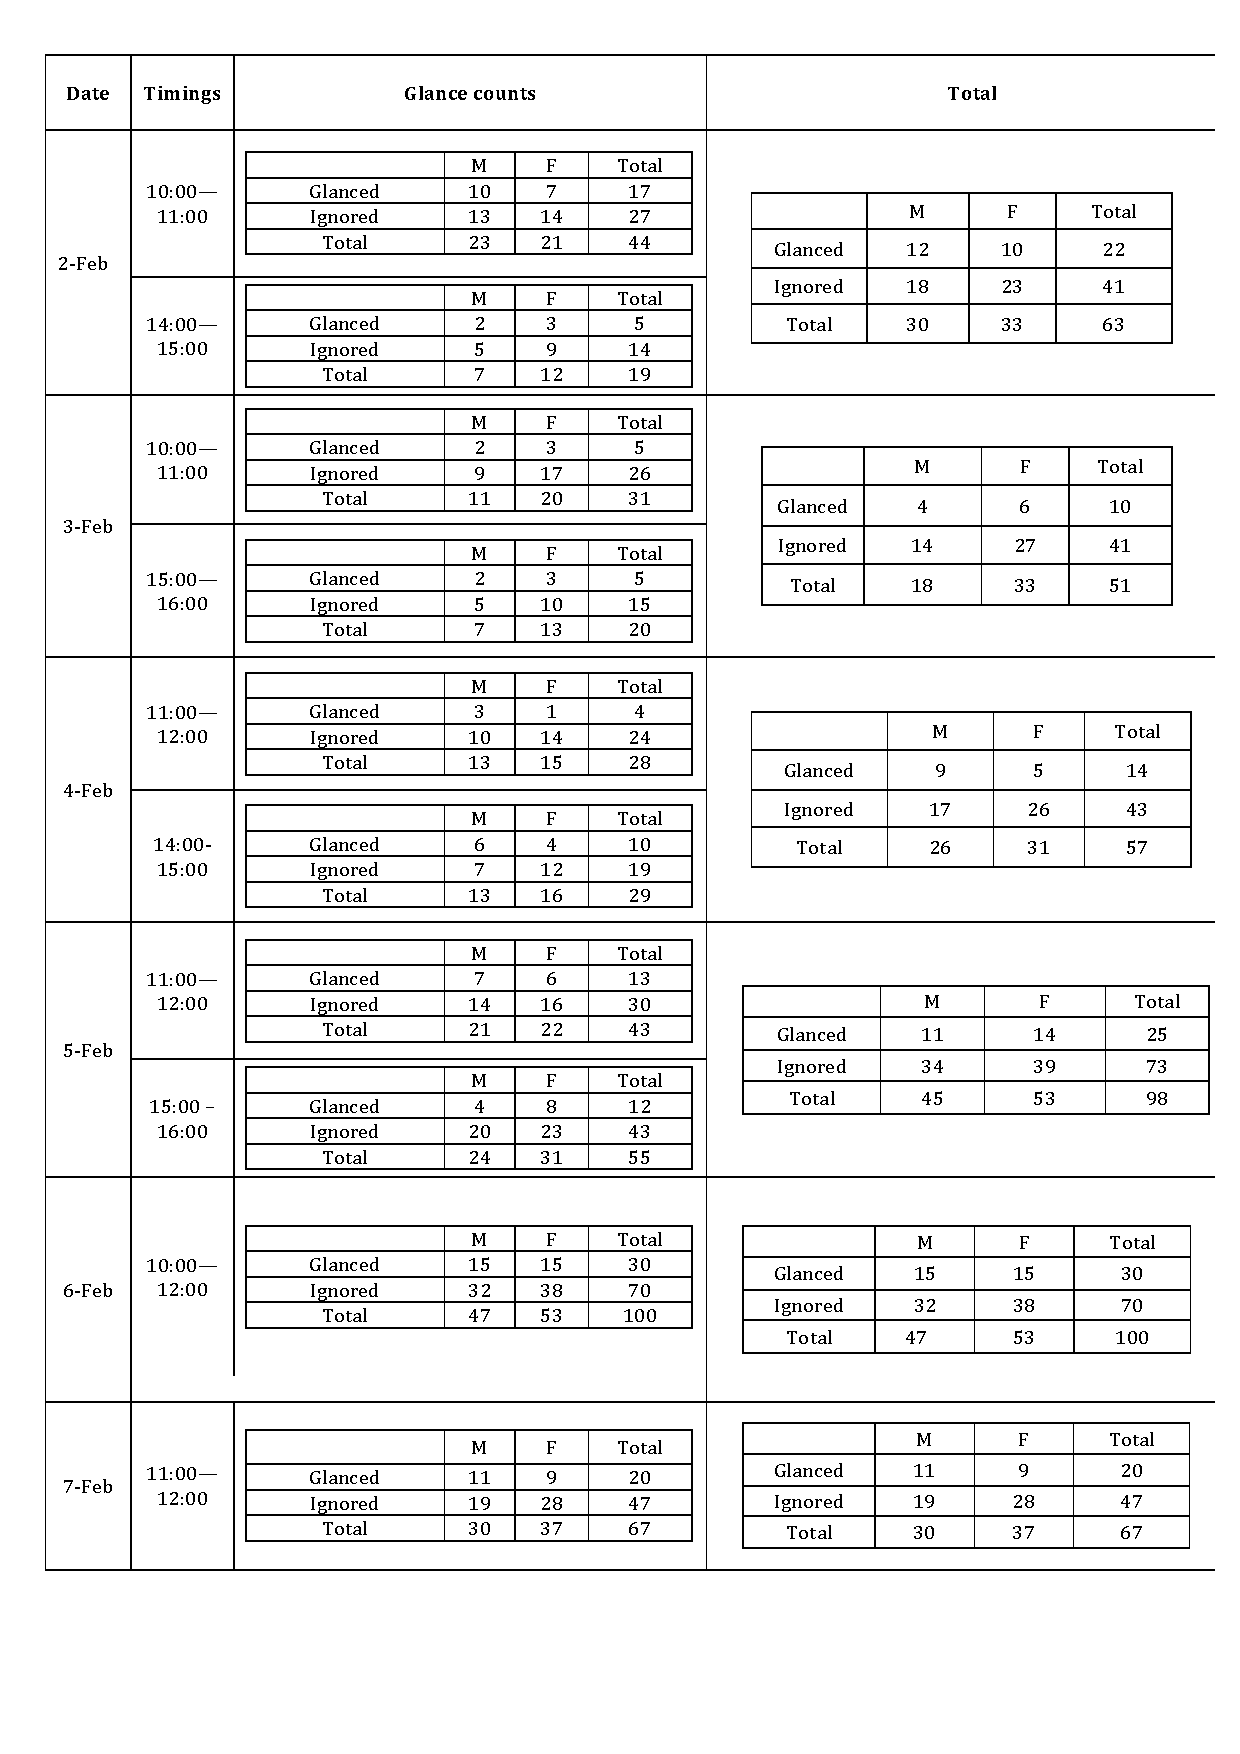
\includepdf[pages=1,width = 20cm, height=22cm,pagecommand=\section{Non-Interactive glance count}]{Appendices/8/non-interactive/non-interactive_glances.pdf}


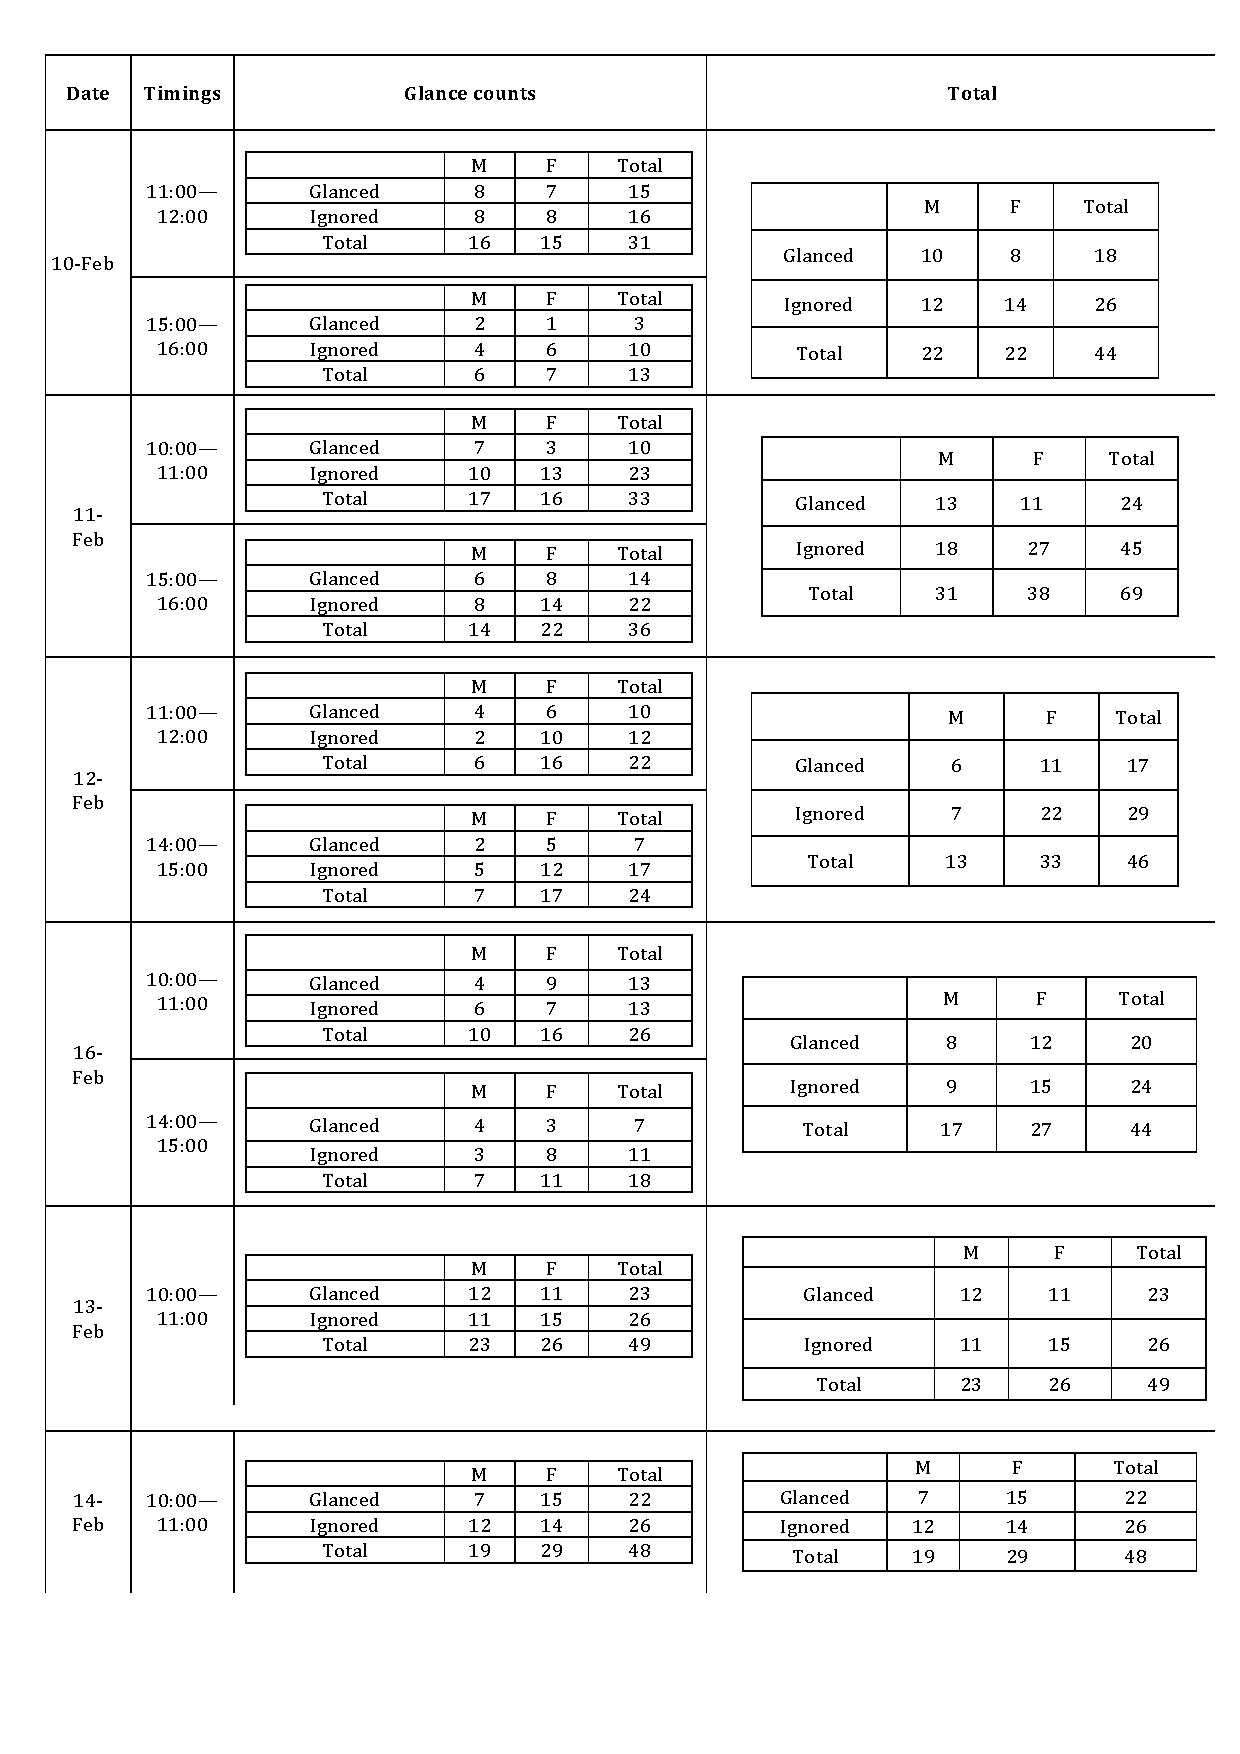
\includepdf[pages=1,width = 20cm, height=22cm,pagecommand=\section{Body Interactive glance count}]{Appendices/8/body-interactive/body-interactive_glances.pdf}


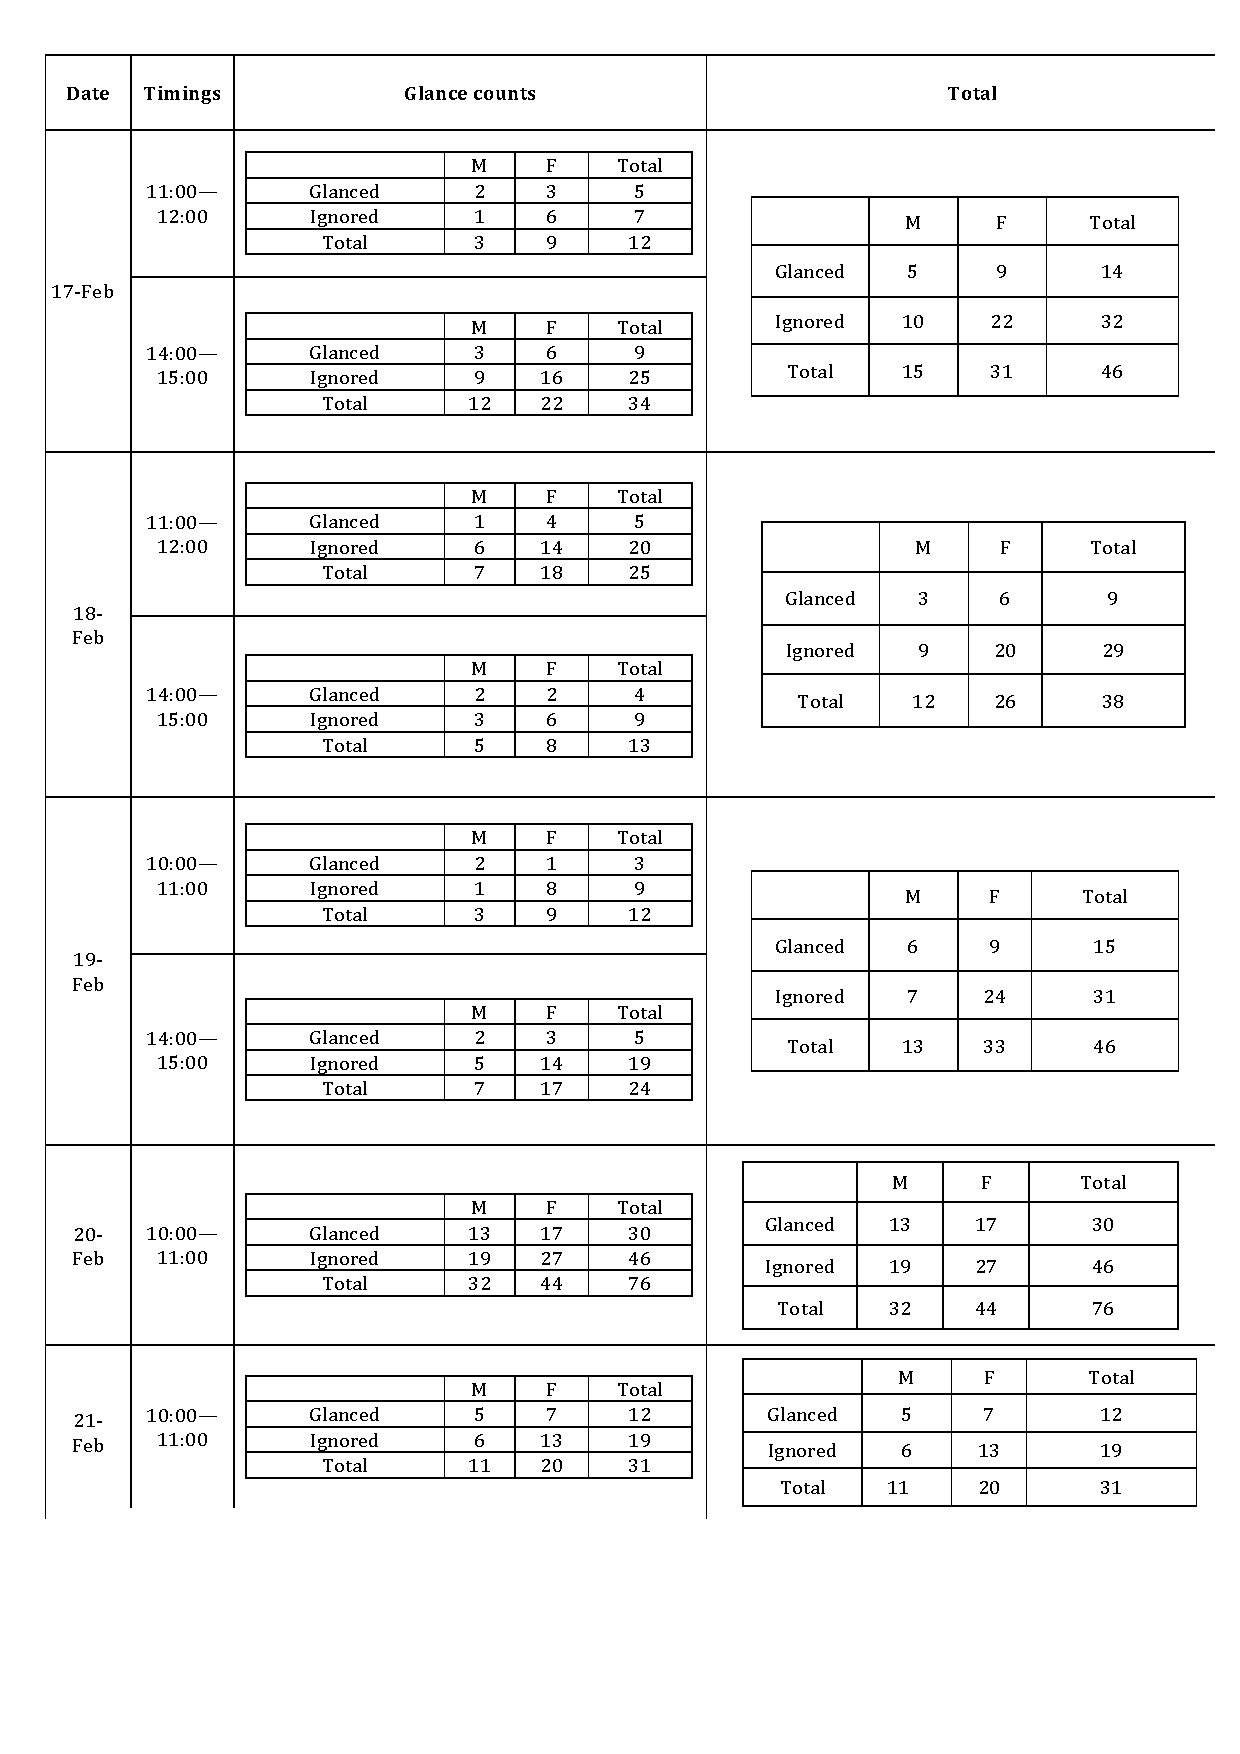
\includepdf[pages=1,width = 20cm, height=22cm,pagecommand=\section{Mobile Interactive glance count}]{Appendices/8/mobile-interactive/mobile-interactive_glances.pdf}



% Interview color code diagrams
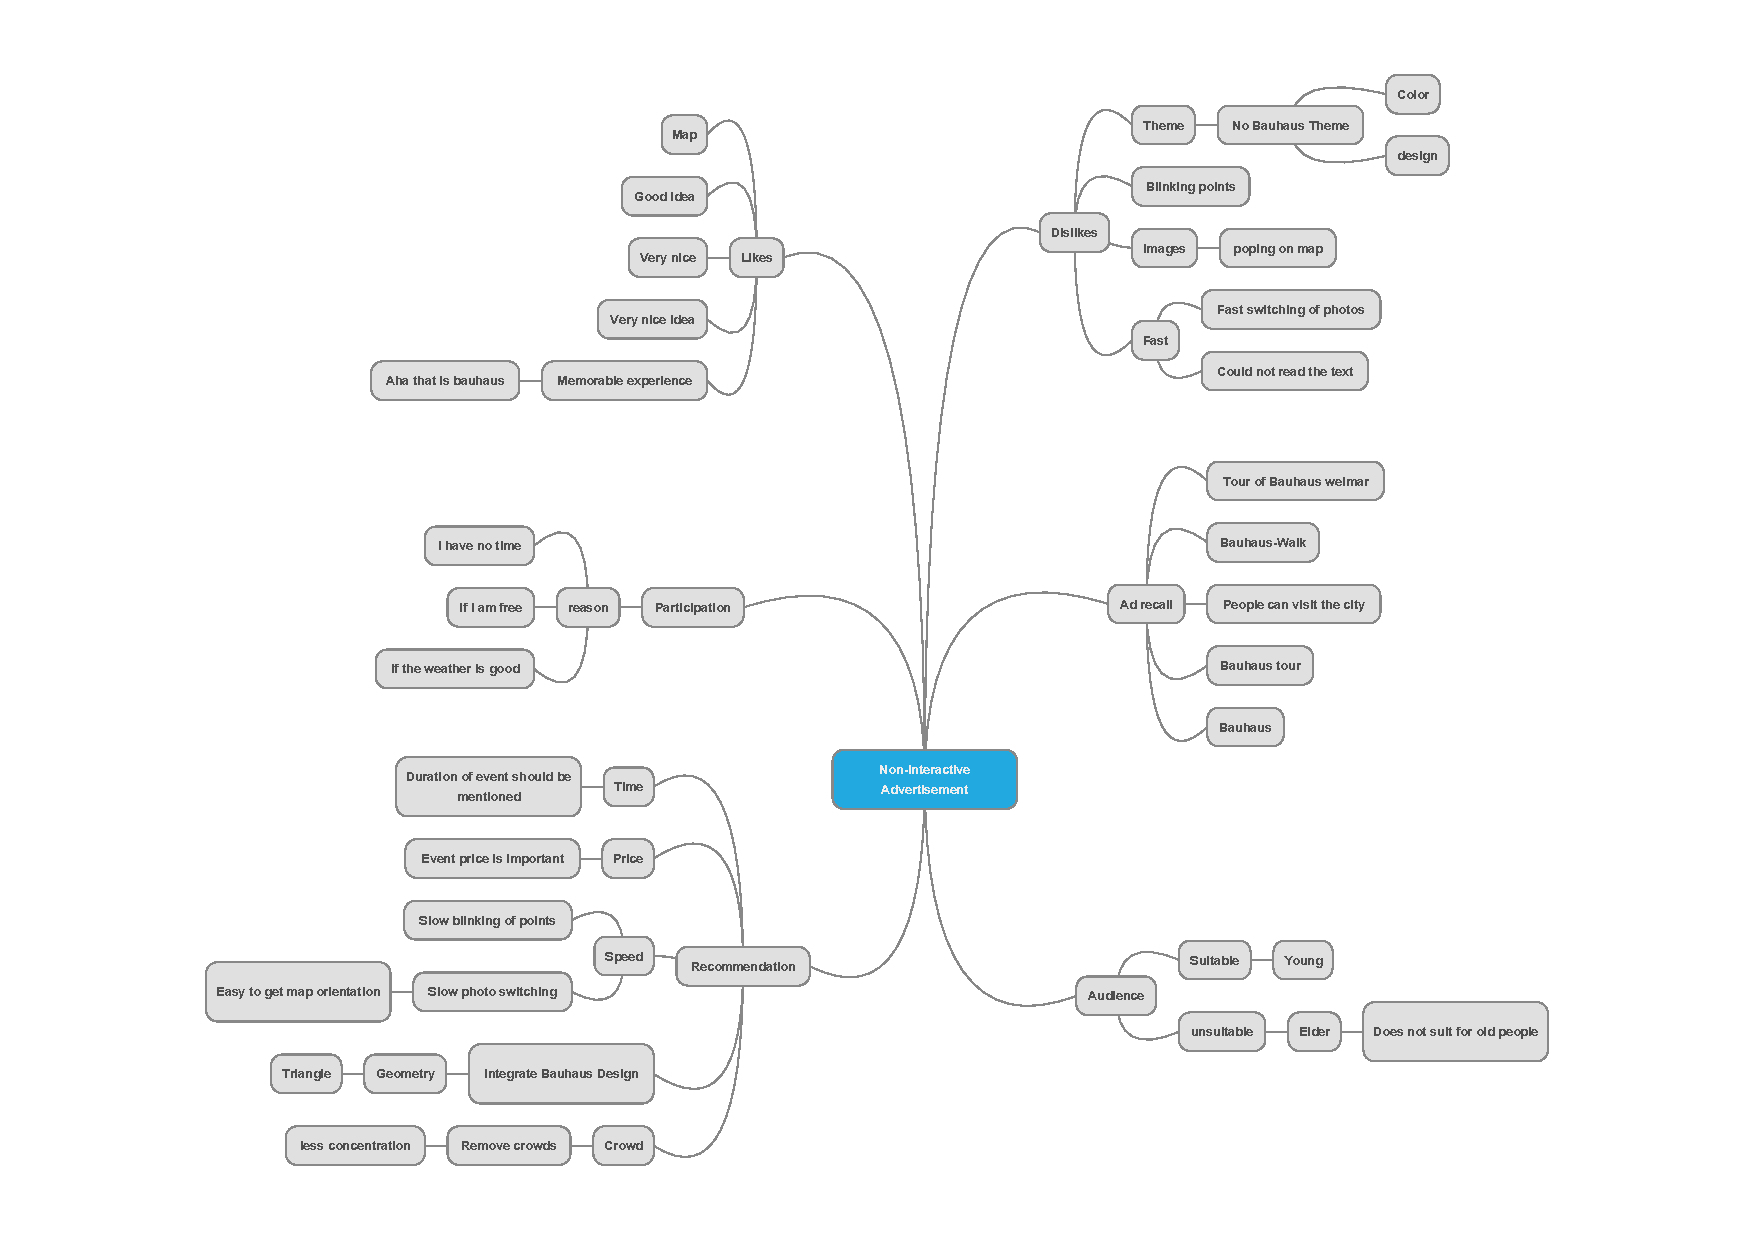
\includepdf[pages=1,width = 20cm, height=22cm,pagecommand=\section{Non-Interactive interview code}]{Appendices/8/non-interactive/non-interactive_code.pdf}

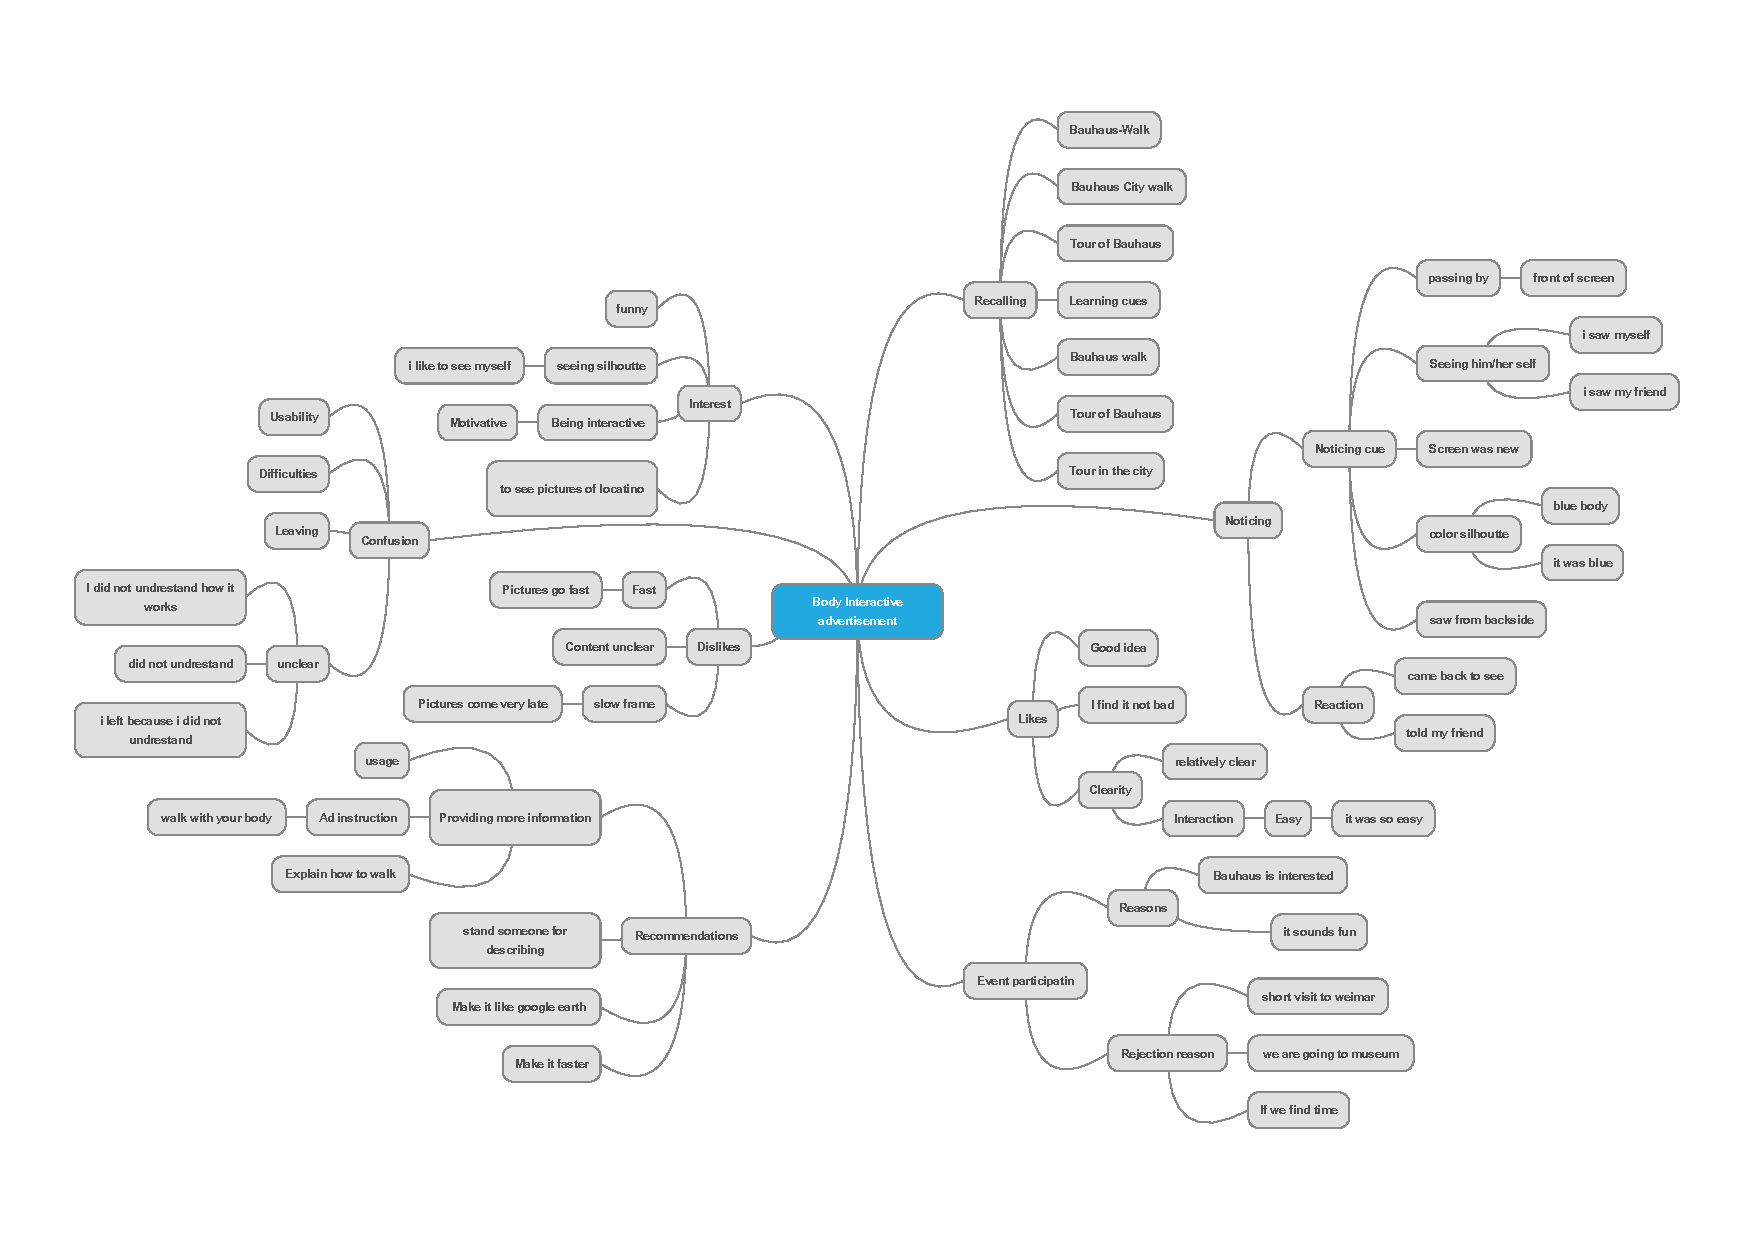
\includepdf[pages=1,width = 20cm, height=22cm,pagecommand=\section{Body Interactive interview code}]{Appendices/8/body-interactive/body-Interactive_code.pdf}

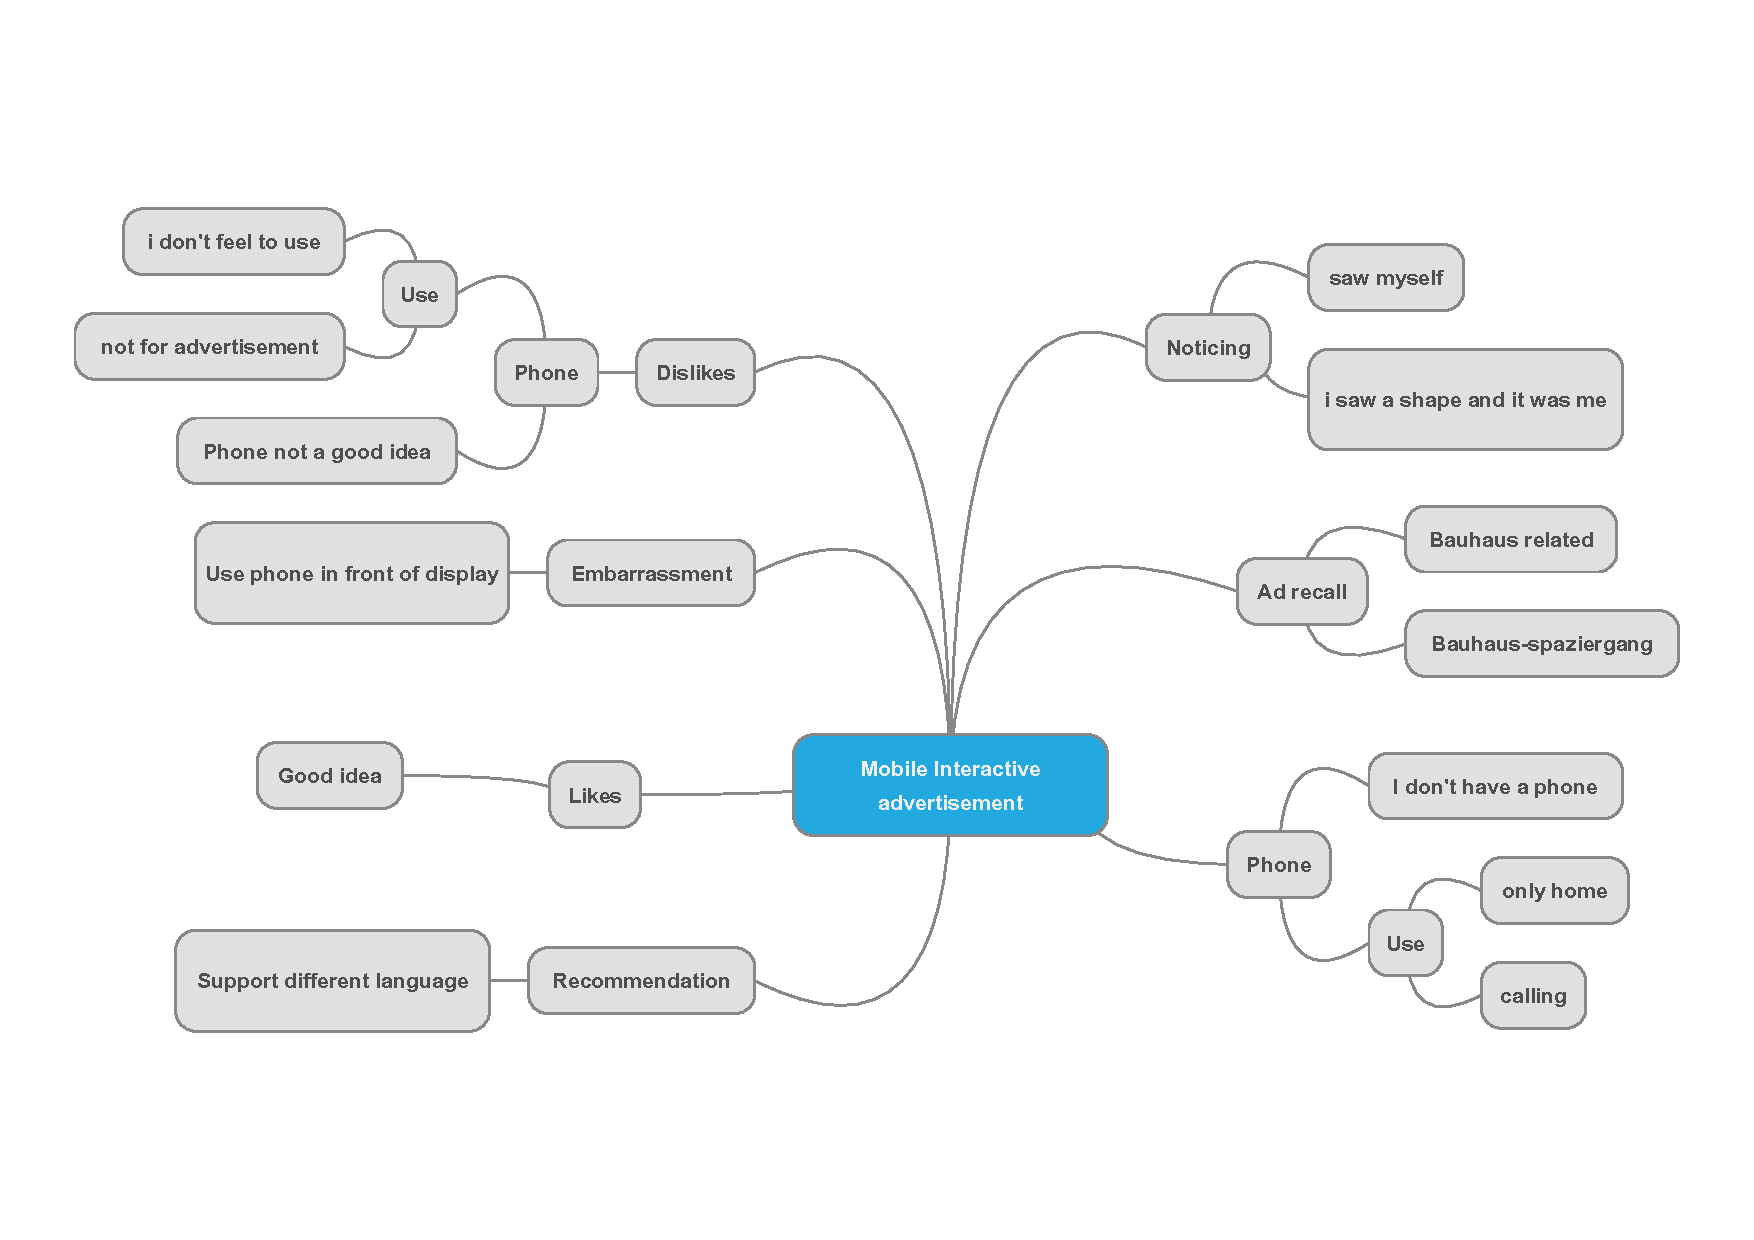
\includepdf[pages=1,width = 20cm, height=22cm,pagecommand=\section{Mobile Interactive interview code}]{Appendices/8/mobile-interactive/mobile-Interactive_code.pdf}


% Observation notes
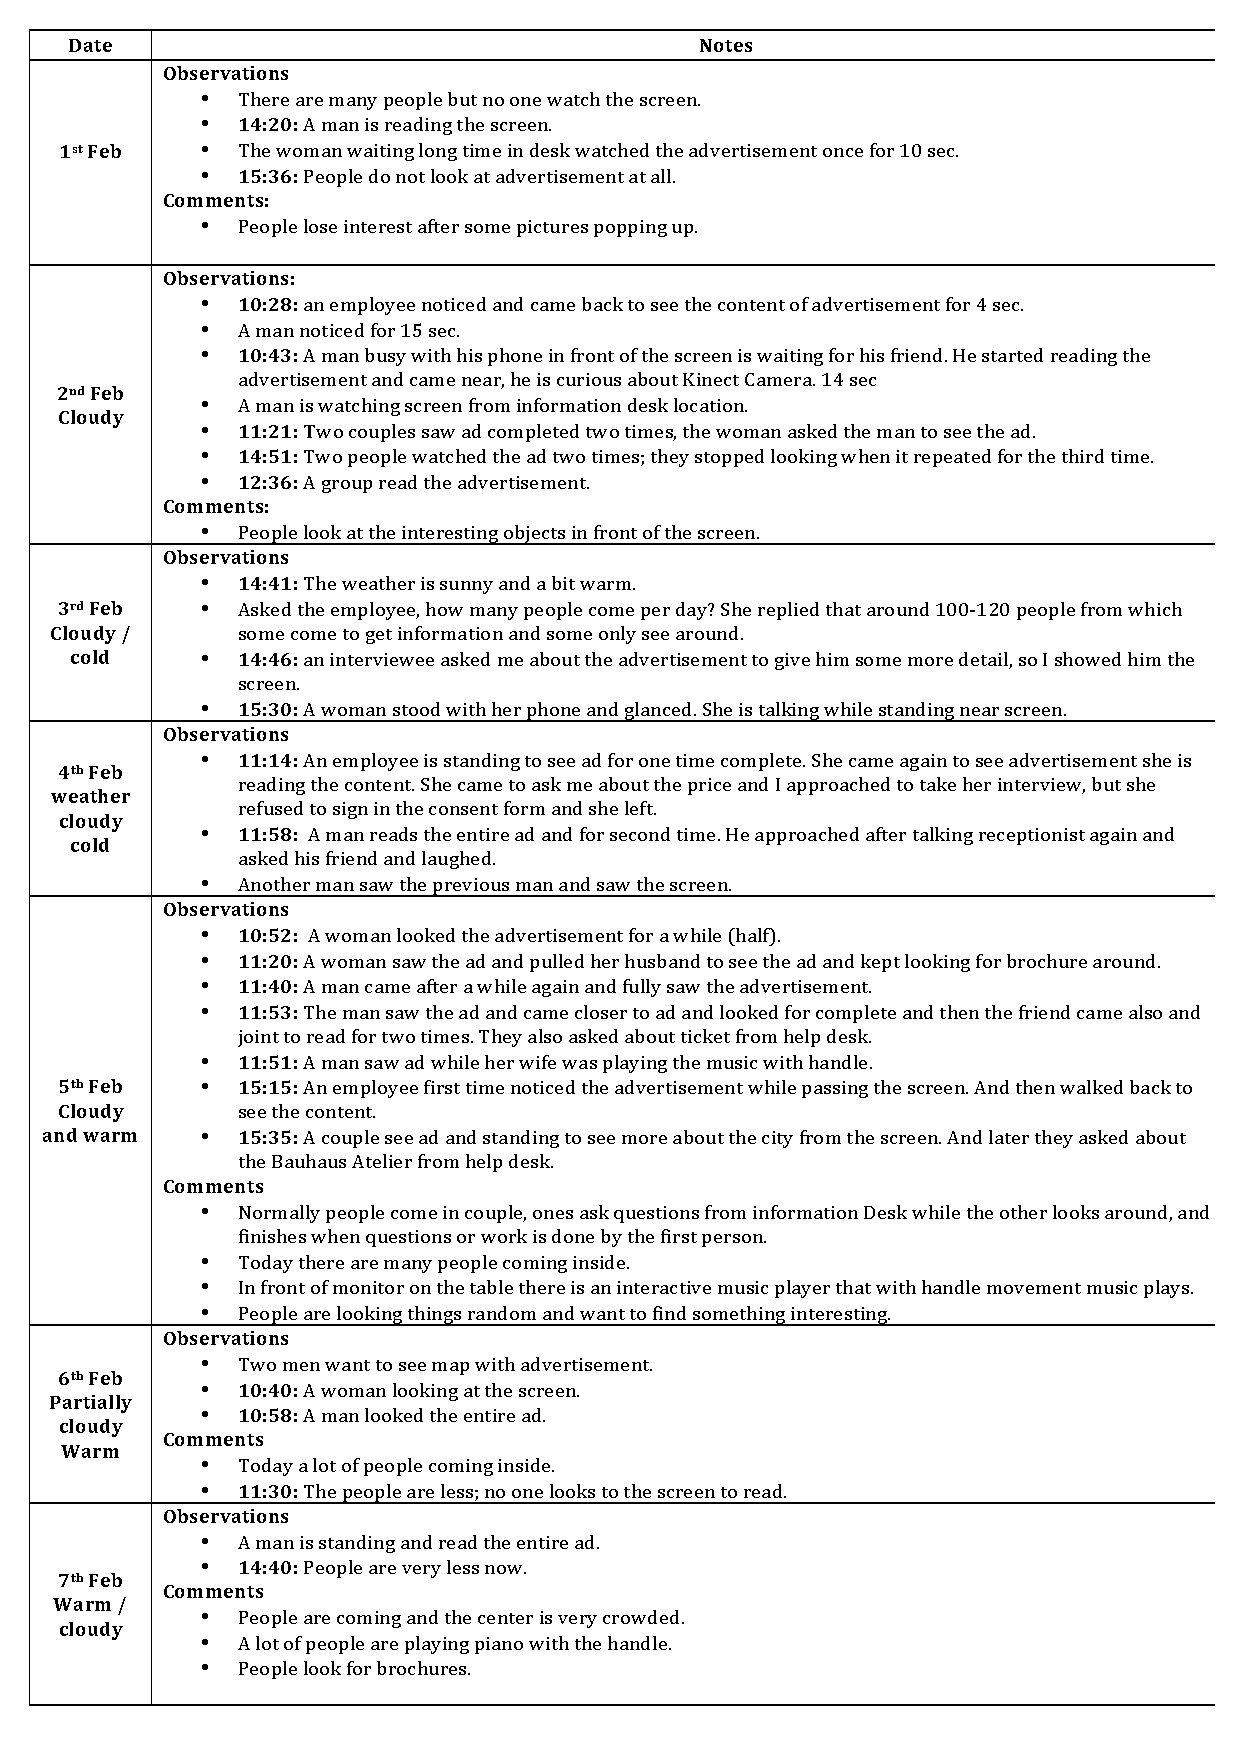
\includepdf[pages=1,width = 15cm, height=22cm,pagecommand=\section{Non-Interactive observation notes}]{Appendices/8/non-interactive/Observation_notes.pdf}

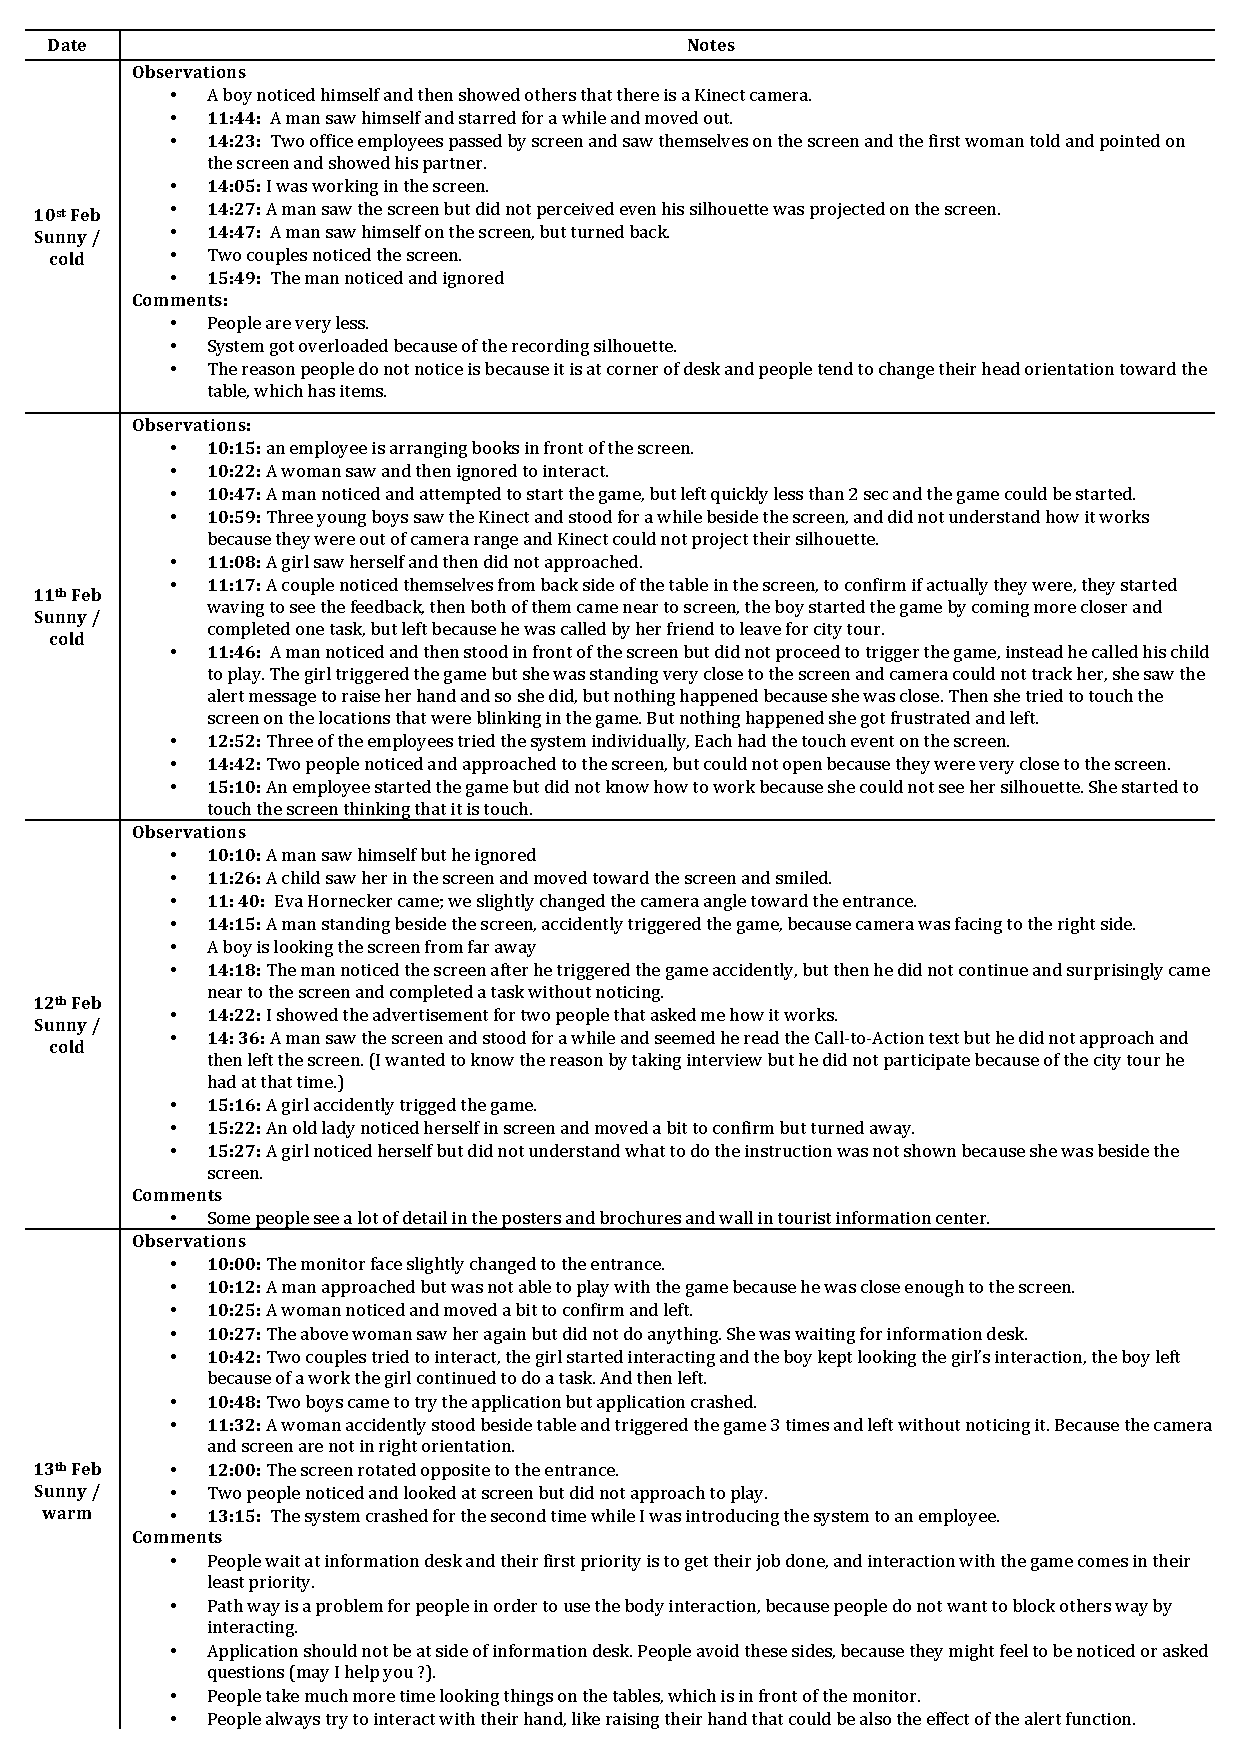
\includepdf[pages=1,width = 15cm, height=22cm,pagecommand=\section{Body Interactive observation notes (1)}]{Appendices/8/body-interactive/Note_1.pdf}

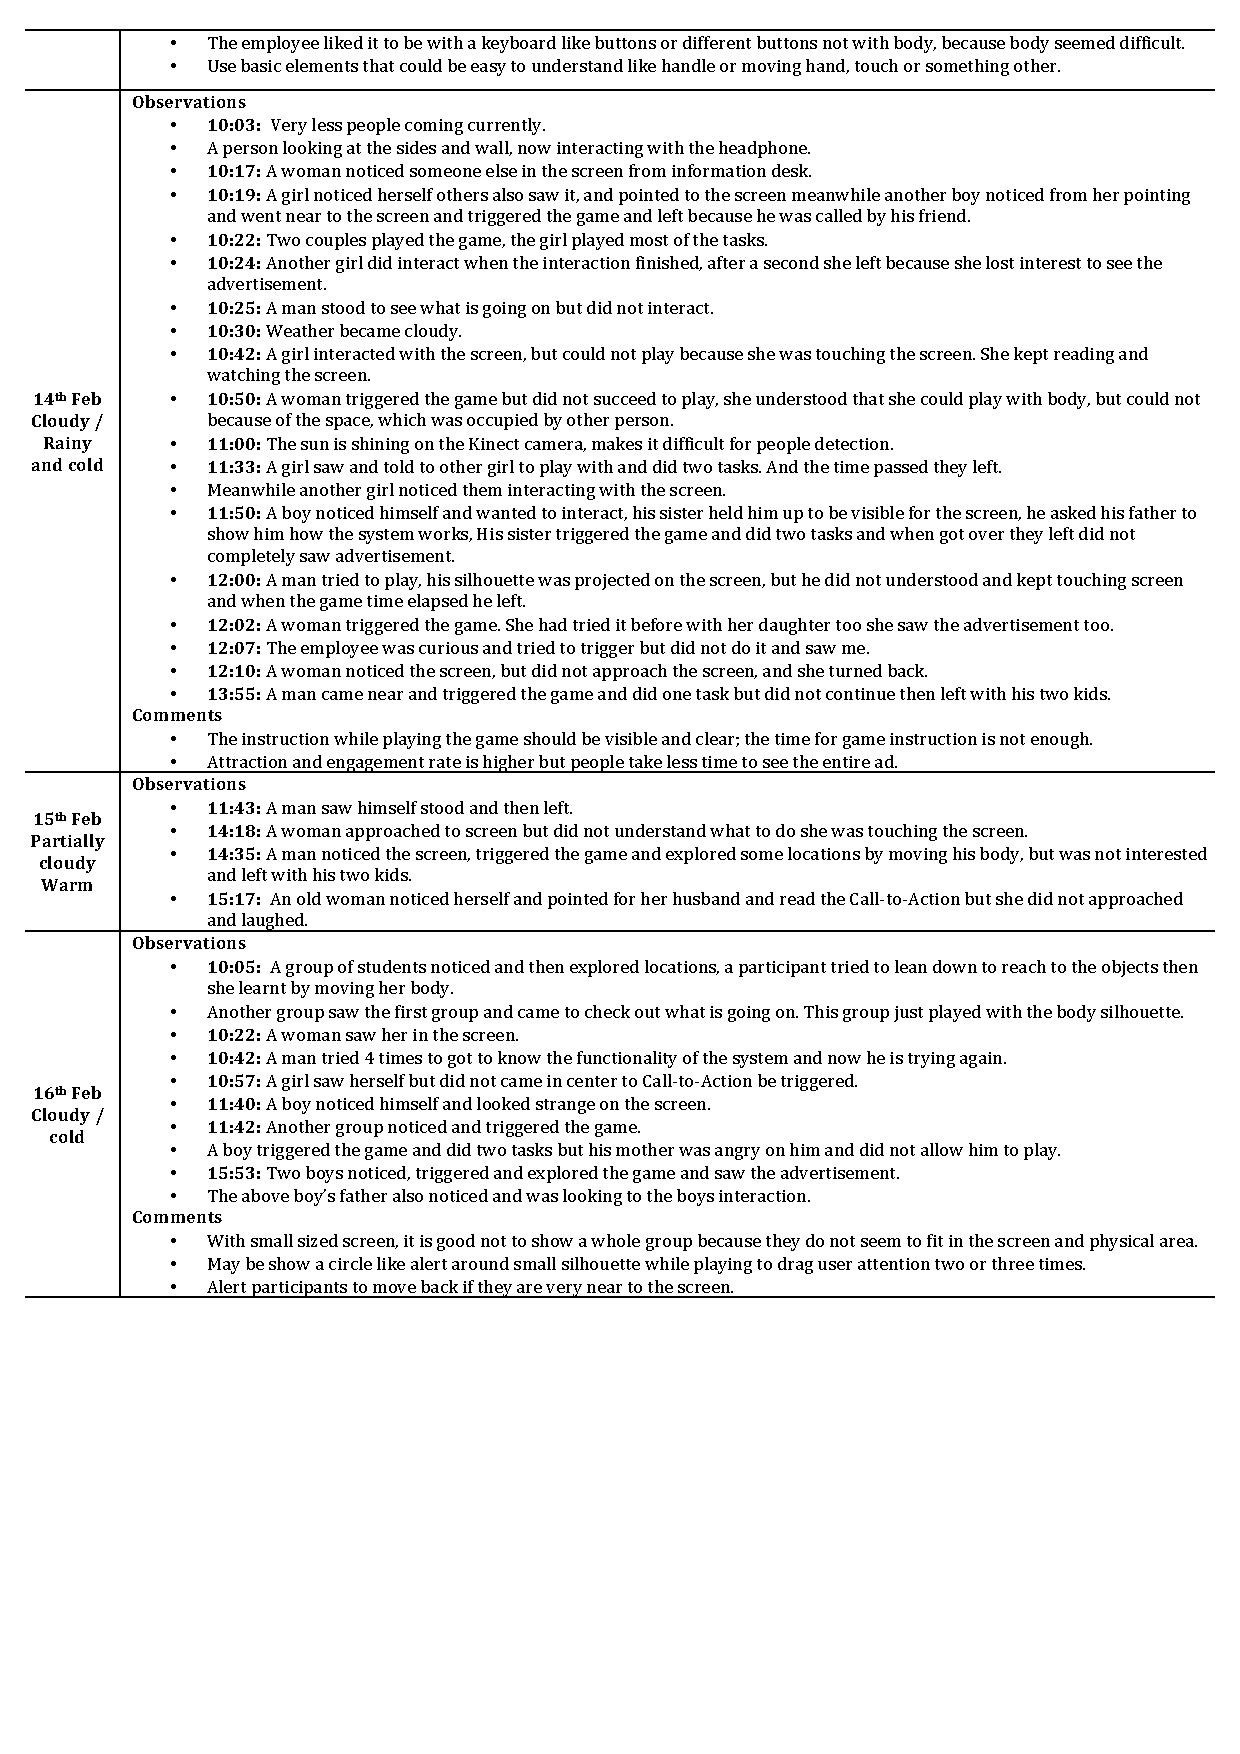
\includepdf[pages=1,width = 15cm, height=22cm,pagecommand=\section{Body Interactive observation notes (2)}]{Appendices/8/body-interactive/Note_2.pdf}


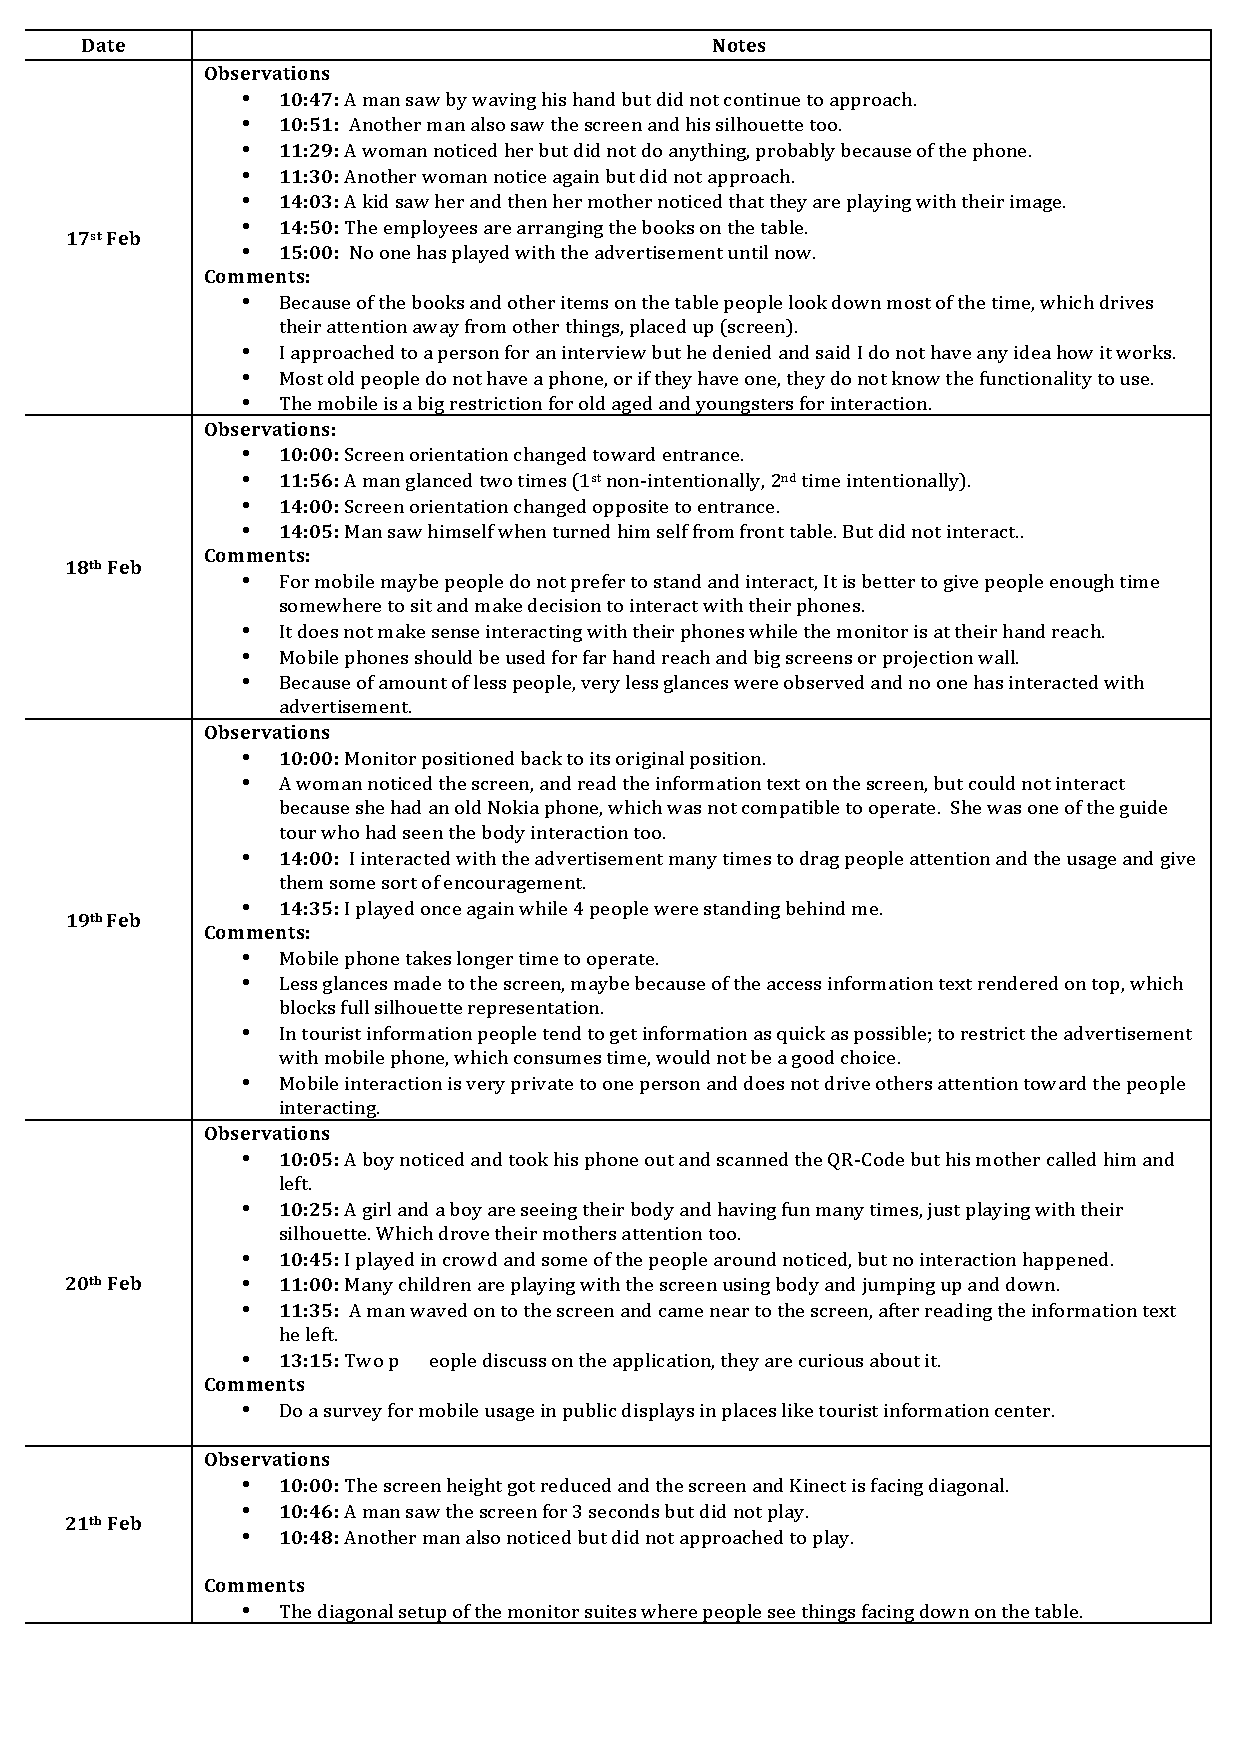
\includepdf[pages=1,width = 15cm, height=22cm,pagecommand=\section{Mobile Interactive observation notes}]{Appendices/8/mobile-interactive/notetaking.pdf}


















